\documentclass{beamer}

\mode<presentation>
{
  \usetheme{Madrid}
  \setbeamercovered{transparent}
}


\usepackage[english]{babel}
\usepackage[utf8]{inputenc}
\usepackage{times}
\usepackage[T1]{fontenc}


\title[Short Paper Title] % (optional, use only with long paper titles)
{Design and Analysis of Plugless Charging of Electric Vehicle using Magnetic Resonance}

\subtitle
{End of semester defense} % (optional)

\author[]{Anjil Adhikari, 073 BEL 307 \\
Praveen Kushwaha, 073 BEL 328 \\
Rabin Dhamala, 073 BEL 329 \\
Rajiv Bijukche, 073 BEL 330 
}
\begin{document}
\frame{\titlepage}
\begin{frame}{Introduction}

\end{frame}

\begin{frame}
  \frametitle{Problem Identification}
\end{frame}

\begin{frame}
\frametitle{Objective}

\end{frame}

\begin{frame}
  \begin{center}
  \frametitle{Block Diagram}
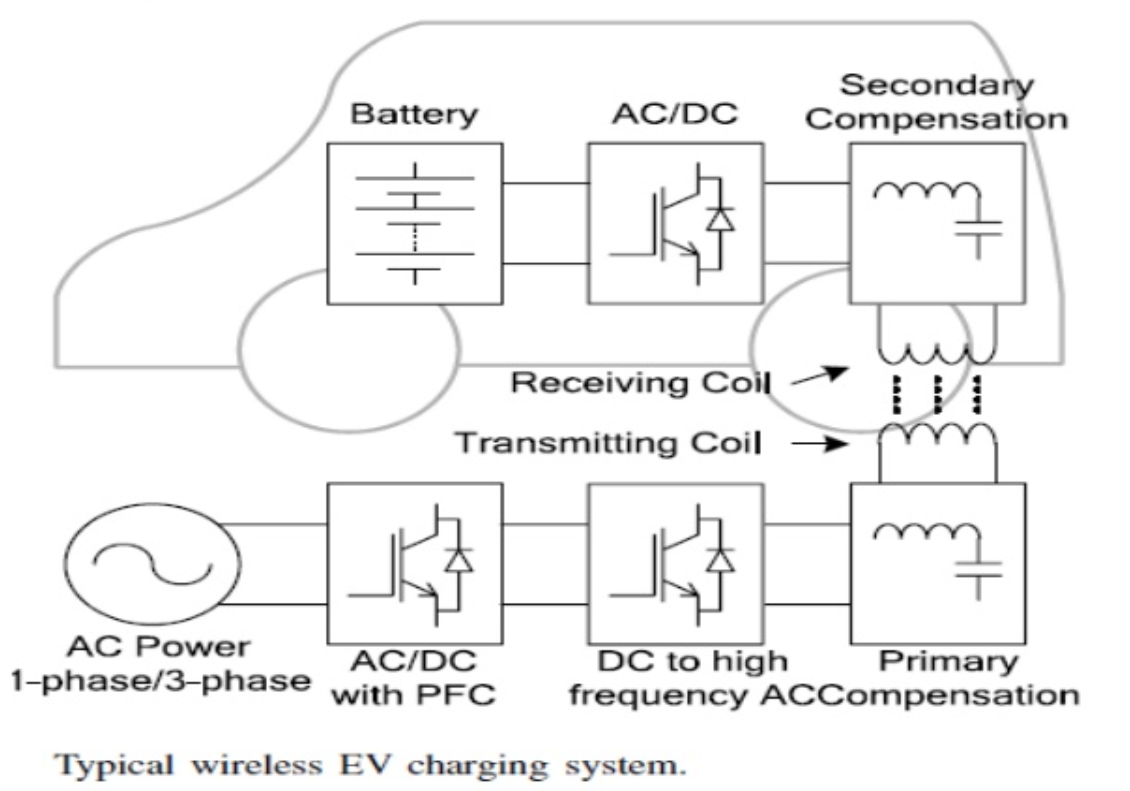
\includegraphics[scale=0.5]{jpgs/wirelessEV.PNG}
  \end{center}
\end{frame}

\begin{frame}
  \frametitle{Work Completed}
  Design of each individual component was completed. Following components were designed
  \begin{itemize}
    \item Rectifier
    \item High frequency inverter
    \item Receiver-Transmitter Coil
    \item Buck Converter
  \end{itemize}
\end{frame}

\begin{frame}
  \frametitle{Rectifer}
  220 V Ac supply was converted into DC voltage using bridge rectifer. Capacitor was used to smoothen the pulsating DC voltage . 

\end{frame}

\begin{frame}
  \frametitle{High Frequency Inverter}

  

\end{frame}
\begin{frame}
  \frametitle{Remaining Work for Next Semester}
  \begin{itemize}
    \item High frequency analysis of receiver transmitter coil using Ansys Maxwell
    \item Hardware realization of prototype of simulated model
  \end{itemize}
\end{frame}

\begin{frame}
  \center
  {\huge ----- END ------}
\end{frame}

\end{document}